\section{Algorithm}
\label{sec:algorithm}

\begin{figure*}[ht!]
  \centering
  \begin{subfigure}[b]{0.33\textwidth}
    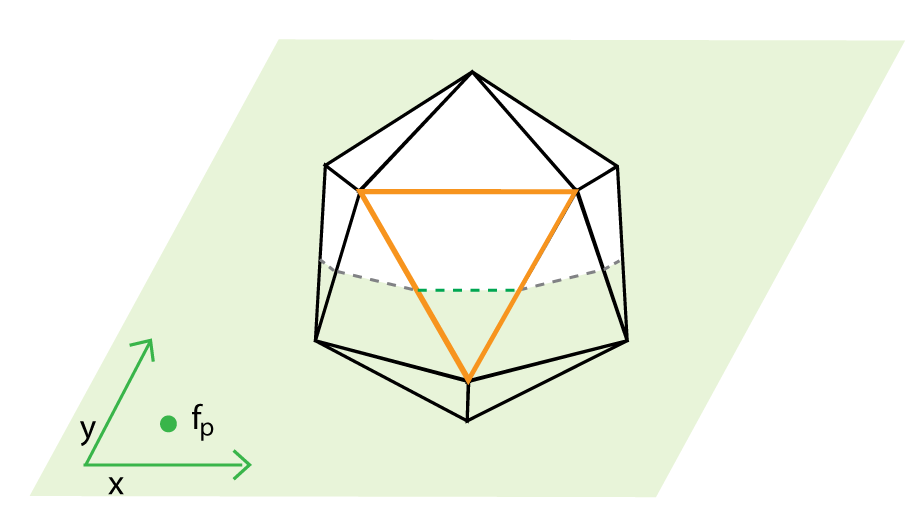
\includegraphics[width=\linewidth]{hsp_mesh-slicing.png}
    \caption{%
      Slicing a mesh
    }
    \label{fig:slicing:mesh}
  \end{subfigure}
  ~
  \begin{subfigure}[b]{0.33\textwidth}
    \centering
    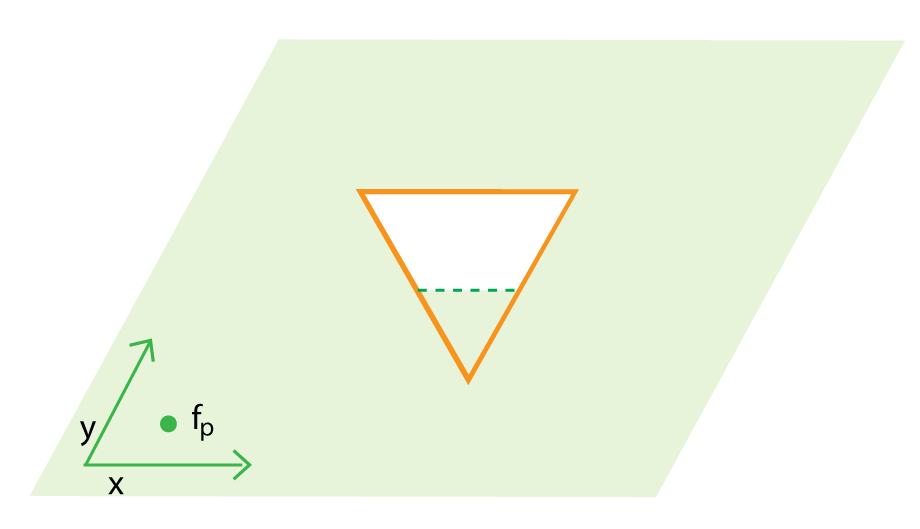
\includegraphics[width=\linewidth]{hsp_simplex-slicing.png}
    \caption{%
      Slicing a simplex
    }
    \label{fig:slicing:simplex}
  \end{subfigure}
  ~
  \begin{subfigure}[b]{0.24\textwidth}
    \centering
    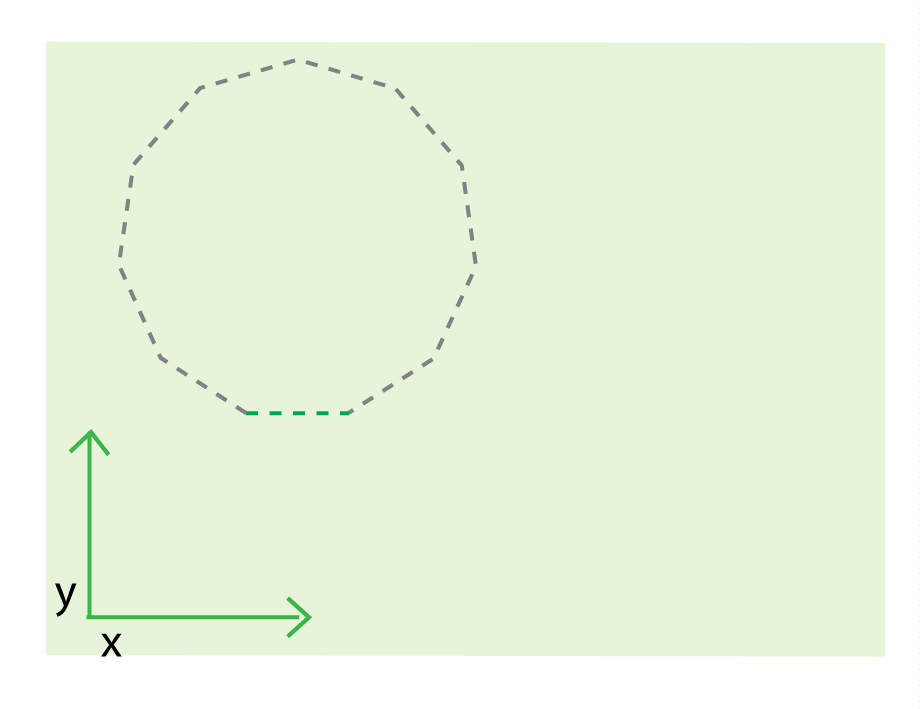
\includegraphics[width=\linewidth]{hsp_plane-slicing.png}
    \caption{%
      2D slice
    }
    \label{fig:slicing:plane}
  \end{subfigure}
  \caption{%
    An overview of how our algorithm functions. The goal is to compute the
    intersection of a slice with a polytope defined as a simplical mesh
    (\subref{fig:slicing:mesh}). The slice is defined by selecting a focus
    point and then extending it in two directions. We 
    (\subref{fig:slicing:simplex}) treat each simplex in the mesh 
    independently and compute the intersection of the simplex with the slice
    (see \autoref{alg:slicing:single}). The collection of all intersections
    for a particular plane is shown as a line plot 
    (\subref{fig:slicing:plane}). This process is repeated over a number of 
    randomly sampled focus points.
  }
  \label{fig:slicing}
\end{figure*}

%Now we turn to how we actually compute a two-dimensional slice of a
%multi-dimesnsional polytope.
There are a several ready-made solutions to creating a number of uniformly
distributed multi-dimensional samples (e.g.\ Sobol sequence~\cite{Sobol:1967}
or Latin hypercube~\cite{Mckay:1979}). These methods are based on ensuring that
the distance between sample points is as even as possible.  These will be our
focus points. Based on this, our main contribution is an algorithm
on how to slice a multi-dimensional polytope.  The algorithm will produce a
single two-dimensional axis-aligned slice for a single focus point. To produce
the full multi-dimensional view we repeat this algorithm for each focus point
and dimension pair.

\subsection{Conceptual overview}

Other slicing techniques, like Sliceplorer~\cite{Torsney-Weir:2017a} or
HyperSlice~\cite{Wijk:1993}, show slices of multi-dimensional manifolds.
In this case we can fix all but one or two of the
parameters, the parameters representing the slice, to a fixed value based on the
focus point. This gives us a two-dimensional function which we can draw as
a one- or two-dimensional function plot.

In our case, we have a simplical hull. This hull can be computed as a convex
hull of a point cloud using an algorithm such as quickhull~\cite{Barber:1996}
or they can be pre-defined.  In either case, a simplical hull is a set of
\(d-1\)-dimensional simplices for a \(d\)-dimensional space. 
A two-dimensional
slice is equivalent to a two-dimensional plane. So, in order to compute the
two-dimensional slice, we need to compute the intersection of a two-dimensional
plane with a set of \(d-1\)-dimensional simplices 
(see \autoref{fig:slicing:mesh}). 

The method often used in graphics for
computing a plane/simplex intersection is to represent the plane as a point and
normal vector. Then, we find the intersection by checking, for each pair of
points, if they are on opposite sides of the plane.
This works for 2D planes (slices) in 3D space
since the normal to the plane is unique. However, in more than three dimensions
we cannot use this method to compute the intersection of a 2D planar object.
This planar object does not have a well-defined concept of a ``side'' in a
multi-dimensional space. The analogy to this is a line in three-dimensions.

Our solution to this problem relies on two key observations. We can treat the
plane as a point with two free parameters and then see if
this point lies on the boundary of the simplex using barycentric coordinates.
A barycentric coordinate defines the location of a point on the face of a simplex.
%The plane must intersect the simplex
%at its boundaries. We express the position of a point within a simplex by using barycentric coordinates. 
For a single focus point, we choose a point somewhere in the domain. Then we
select two axis-aligned directions and create a plane by setting the values
of that point to free parameters, which we denote $x$ and $y$. These free parameters
create a 2D plane. We then want to see where this plane intersects the simplex
(\autoref{fig:slicing:simplex}). 
A point is located on the boundary of a simplex whenever at least one
barycentric coordinate is zero and the rest are between zero and one. 
If there is a solution then we will have a formula for the line segment
through the simplex (\autoref{alg:slicing:single}).
We compute these line segments for each plane/simplex intersection. The
collection of intersecting lines forms the image of the slice on the plane
(see \autoref{fig:slicing:plane}).

The simplical hull of a shape consists of $d−1$-dimensional simplices. However, in
order to convert to barycentric coordinates without using a pseudoinverse we
need a $d$-dimensional simplex where every point has a unique representation.
Therefore, we add the focus point as an extra vertex.  Now we have a
$d$-dimensional simplex. This will lead us to a square matrix, which is easy to
invert.  Any intersections with the extra point are removed at the end of the
algorithm.

\subsection{Algorithm details}

The algorithm requires that the shape we are slicing is specified as a set of
simplices. Each combination of simplex, pair of slicing dimensions, and focus
point is handled independently. These can be looped through, as in the
pseudocode (see \autoref{alg:slicing:all}), or in parallel, as in our actual
implementation.

To illustrate how our slicing algorithm works we first introduce some notation.  We begin with a $d$-dimensional focus point $f_p$ and a simplex $s$
consisting of $d+1$ $d$-dimensional points, $x_1, \ldots, x_{d+1}$. We denote
the slice as $f_p'$ in the formulas below. Without loss of generality, we will
assume the slicing dimensions to be $(d_1,d_2)=(1,2)$. Then, the two free
variables for the specification of the slice, $x$ and $y$, will replace the
first two components of the focus point (\autoref{eq:fp}). 
%\msnote{we might want to include 
%equations right at the spot. Imho this makes it easier to read. But maybe just a matter of style/taste ...}
We let $T$
be the matrix to convert a point from barycentric coordinates to Cartesian
coordinates (including a homogeneous component of 1). The columns of $T$ are the $d+1$ points defining the simplex. We append
a row of ones to ensure that the barycentric coordinates sum to one. The inverse
of $T$ will convert a point from Cartesian coordinates (including a homogeneous component of 1) back to barycentric coordinates.

\begin{align}
  f_p &= [p_1, p_2, \ldots, p_d,1] \\
  f'_p &= [x, y, p_3, \ldots, p_d, 1] \label{eq:fp} \\
  T &= 
    \begin{bmatrix}
      x_{1,1} & x_{2,1} & \cdots & x_{d+1,1} \\
      x_{1,2} & x_{2,2} & \cdots & x_{d+1,2} \\
      \vdots  & \vdots  & \ddots & \vdots    \\
      x_{1,d} & x_{2,d} & \cdots & x_{d+1,d} \\
      1       & 1       & \cdots & 1         
    \end{bmatrix} \\
\end{align}

The next step is to convert the slice, $f_p'$, to barycentric coordinates, 
$\lambda$.
\begin{align}
  T^{-1} &= 
    \begin{bmatrix}
      \alpha_{1,1} & \alpha_{2,1} & \cdots & \alpha_{d+1,1} \\
      \alpha_{1,2} & \alpha_{2,2} & \cdots & \alpha_{d+1,2} \\
      \vdots  & \vdots  & \ddots & \vdots    \\
      \alpha_{1,d+1} & \alpha_{2,d+1} & \cdots & \alpha_{d+1,d+1}
    \end{bmatrix} \\
  \lambda &= T^{-1} f'_p \\
          &= 
    \begin{bmatrix}
      \alpha_{1,1} x &+ \alpha_{2,1} y &+ \alpha_{3,1} p_3 &+ \cdots &+ \alpha_{d+1,1} \\
      \alpha_{1,2} x &+ \alpha_{2,2} y &+ \alpha_{3,2} p_3 &+ \cdots &+ \alpha_{d+1,2} \\
      \vdots \\
      \alpha_{1,d+1} x &+ \alpha_{2,d+1} y &+ \alpha_{3,d+1} p_3 &+ \cdots &+ \alpha_{d+1,d+1} \\
    \end{bmatrix}
    \label{eq:inverted}
\end{align}
This equation is essentially a linear equation in $x$ and $y$ and we denote its coefficients by $\lambda_x$, $\lambda_y$, and $\lambda_c$ respectively.
%If we look at $\lambda$, we will see that since there are two free parameters,
%each component of $\lambda$ will have a coefficient of $x$, coefficient of $y$,
%and a constant part. We let $\lambda_x$, $\lambda_y$, and $\lambda_c$ be each
%of these numbers respectively. 
Thus, each component is an equation of a line ($t$ is denoting the transpose).
\begin{align}
  \lambda_x &= \left[ \alpha_{1,1}, \alpha_{1,2}, \ldots, \alpha_{1,d+1} \right]^t \\
  \lambda_y &= \left[ \alpha_{2,1}, \alpha_{2,2}, \ldots, \alpha_{2,d+1} \right]^t \\
  \lambda_c &= \left[ \sum_{i=3}^{d+1} \alpha_{i,1} p'_i, \ldots, \sum_{i=3}^{d+1} \alpha_{i,d+1} p'_{d+1} \right]^t \\
  \lambda &= \lambda_x x + \lambda_y y + \lambda_c
\end{align}

Here, $x$ and $y$ correspond to the horizontal and vertical coordinates of the
intersection of the plane with the simplex. Each component of $\lambda$
reflects the influence of one of the ($d+1$) points of the simplex. If the
influence is zero (i.e. for the $i$-th point we have $\lambda_i=0$) then we are on
the boundary of the simplex.  An intersection of a plane with a
simplex must cross the boundaries
(\autoref{fig:slicing:simplex}) so it suffices to turn each
component of $\lambda$, $\lambda_i$, to zero in turn.  It is possible that the plane will
intersect multiple faces so we set each component of $\lambda$ to $0$ in turn
and then check what range of $x$ and $y$ in the remaining components are valid
barycentric coordinates (i.e.\ are between zero and one).  If this is the case,
then the plane intersects the simplex.  Otherwise, there is no intersection. In
other words, if we are trying to find the intersection for face $i$, we need to
solve $\lambda_i = 0$ such that $\forall j \ne i$, $0 \le \lambda_j \le 1$.
This can be solved either with a linear constraint solver or directly by
solving for $y$ setting $\lambda_i = 0$ and substituting it into each row $j$ of \autoref{eq:inverted}
%$\lambda_j$ 
and then finding an interval for $x$ and $y$ that allows each
$\lambda_j$ to be between $0$ and $1$.  We can do this by individually finding
the valid $x, y$ interval for each $j$ and then taking the intersection of all the
individual intervals. If the intersection is non-empty then this is the interval
of values for $x$ in the intersection. We can substitute this to find the
interval of values for $y$. We can then draw these intervals as line segments
on the screen (\autoref{fig:slicing:plane}). 

\begin{algorithm}
  \caption{Slicing a single simplex}
  \label{alg:slicing:single}
  \begin{algorithmic}
    \Function{slice}{$p$, $s$, $d_1$, $d_2$}
      \State $T\gets \left[ s\ 1 \right]^t$ \Comment{from barycentric to Cartesian coordinates}
      \State $r \gets p$
      \State $r[d_1,d_2] \gets [x,y]$
      %\State $r_c\gets p$ 
      %\State $r_c[d1,d2]\gets 0$
      %\State $r_x\gets \textbf{0}$
      %\State $r_y\gets \textbf{0}$
      %\State $r_x[d1]\gets 1$
      %\State $r_y[d2]\gets 1$
      %\State $\lambda_c \gets T^{-1} r_c$
      %\State $\lambda_x \gets T^{-1} r_x$
      %\State $\lambda_x \gets T^{-1} r_y$
      \State $\lambda_x x + \lambda_y y + \lambda_c \gets T^{-1} r$ \Comment{convert to barycentric coordinates}
      \State $\textrm{rng}_x \gets [-\infty,\infty]$
      \State $\textrm{rng}_y \gets [-\infty,\infty]$
      \For {$i\gets 1 \textrm{ to } d+1$} \Comment{each face of the simplex} 
        \State $(\textrm{rng}'_x,\textrm{rng}'_y) \gets$ \Call{solve}{$\lambda_{x,i} x + \lambda_{y,i} y + \lambda_{c,i} = 0, \textrm{s.t.} \forall j \ne i, 0 \le \lambda_{x,j} x + \lambda_{y,j} y + \lambda_{c,j} \le 1$}
        \State $\textrm{rng}_x \gets \textrm{rng}_x \cap \textrm{rng}'_x$
        \State $\textrm{rng}_y \gets \textrm{rng}_y \cap \textrm{rng}'_y$
      \EndFor
      \State \Return $\left( \textrm{rng}_x, \textrm{rng}_y \right)$
    \EndFunction
  \end{algorithmic}
\end{algorithm}

\begin{algorithm}
  \caption{Finding slices for all simplices}
  \label{alg:slicing:all}
  \begin{algorithmic}
    \For {$d_1=1 \textrm{ to } d-1$}
      \For {$d_2=d_1 \textrm{ to } d$} \Comment{all pairs of dimensions}
        \State $\textrm{slices} \gets [\varnothing,\varnothing,\varnothing,\varnothing]$ \Comment{4 column matrix for min/max $x$ and $y$}
        \For {$p \in FP$} \Comment{all focus points}
          \For {$s \in S$} \Comment{all simplices}
            \State $\textrm{ranges} \gets$ \Call{slice}{$p$, $s$, $d_1$, $d_2$}
            \If {$\textrm{ranges} \ne \emptyset$} \Comment{add new row if we found an intersection}
              \State $\textrm{slices} \gets \left[ \begin{matrix} \textrm{slices} \\ \textrm{ranges} \end{matrix} \right]$
            \EndIf
          \EndFor
        \EndFor
        \State \Call{plot}{$\textrm{slices}, d_1, d_2$} \Comment{plot slices to proper subplot}
      \EndFor
    \EndFor
  \end{algorithmic}
\end{algorithm}

